\documentclass[9pt,a4paper]{report}
\usepackage{mwe}
\usepackage{listings}
\usepackage{amsmath}
\usepackage{graphicx}
\usepackage{subfig}
\usepackage{float}
\usepackage{xcolor}
\usepackage{multirow}
\usepackage{hyperref}
\usepackage{fancyhdr}
\usepackage{sectsty}
\usepackage[dvipsnames]{xcolor}
\usepackage{soul}
\usepackage[compact]{titlesec}
\usepackage{float}
\usepackage[left=0.5cm,right=0.5cm,top=0.5cm,bottom=0.5cm]{geometry}
\graphicspath{{Series Reverse-breakdown Zener Diode Circuit}}

\newcommand*{\nchapter}[1]{%
	\chapter*{#1}%
	\addcontentsline{toc}{chapter}{#1}
	\vspace{-14mm}}
\newcommand*{\nsection}[1]{%
	\section*{#1}%
	\addcontentsline{toc}{section}{#1}}
\newcommand*{\nsubsection}[1]{%
	\subsection*{#1}%
	\addcontentsline{toc}{subsection}{#1}}
\newcommand*{\nsubsubsection}[1]{%
	\subsubsection*{#1}%
	\addcontentsline{toc}{subsubsection}{#1}}

\chaptertitlefont{\large}
\sectionfont{\normalsize}
\fontsize{9}{11}\selectfont
\begin{document}
	\begin{titlepage}
		\centering
		\vspace*{1.5in}
		
\includegraphics[width=0.15\textwidth]{W-Logo_Purple_RGB}\par\vspace{1cm}
		{\LARGE \textsc{University of Washington}\par}
		\vspace{1cm}
		{\Large \textsc{BEE331 Lab 1.2}\par}
		\vspace{1.5cm}
		{\huge\bfseries \par}
		\vspace{2cm}
		{\Large\itshape 2301991\hspace{55pt}1900585\par}
		{\Large\itshape Jason Truong\hspace{31pt}Henry Haight\par}
		\vfill
		supervised by\par
		Prof.~Joseph \textsc{Decuir}
		\date{2024\\ January}
		\vfill
		% Bottom of the page
		{\large \today\par}
		\vspace*{1.5in}
	\end{titlepage}
	
	\nchapter{Characterising Zener Diodes; I-V Curve}
	\nsection{Design Objective}
	In this lab, we introduce ourselves to the \emph{Zener} diode, we characterise its function by the I-V curve.
	\begingroup
	\renewcommand{\cleardoublepage}{}
	\renewcommand{\clearpage}{}
	\nsection{Circuit Design Outline}
	\endgroup
	With a resistor of an arbitrary impedance greater than $100\Omega$ ($R\geq100\Omega$), and the natural impedance of the Function Generator in series ($R_{TOT}=R_{FG}+R\geq150\Omega$), the (1N4732 or 1n5223) Zener diode is set in series set in reverse-polarity to procate reverse-breakdown from the diode; through the function generator. Set the function generator @ f=1kHz and $V_P=5V$ (We'll be focusing on the negative portion of $V_P$).
	\begin{figure}[hp!]
		\centering
		\caption{\centering Series $R$ + Diode $D_Z$}
		\subfloat[\centering LTSpice + Rudimentary Schematic Series RD ($499\Omega$) Circuit]{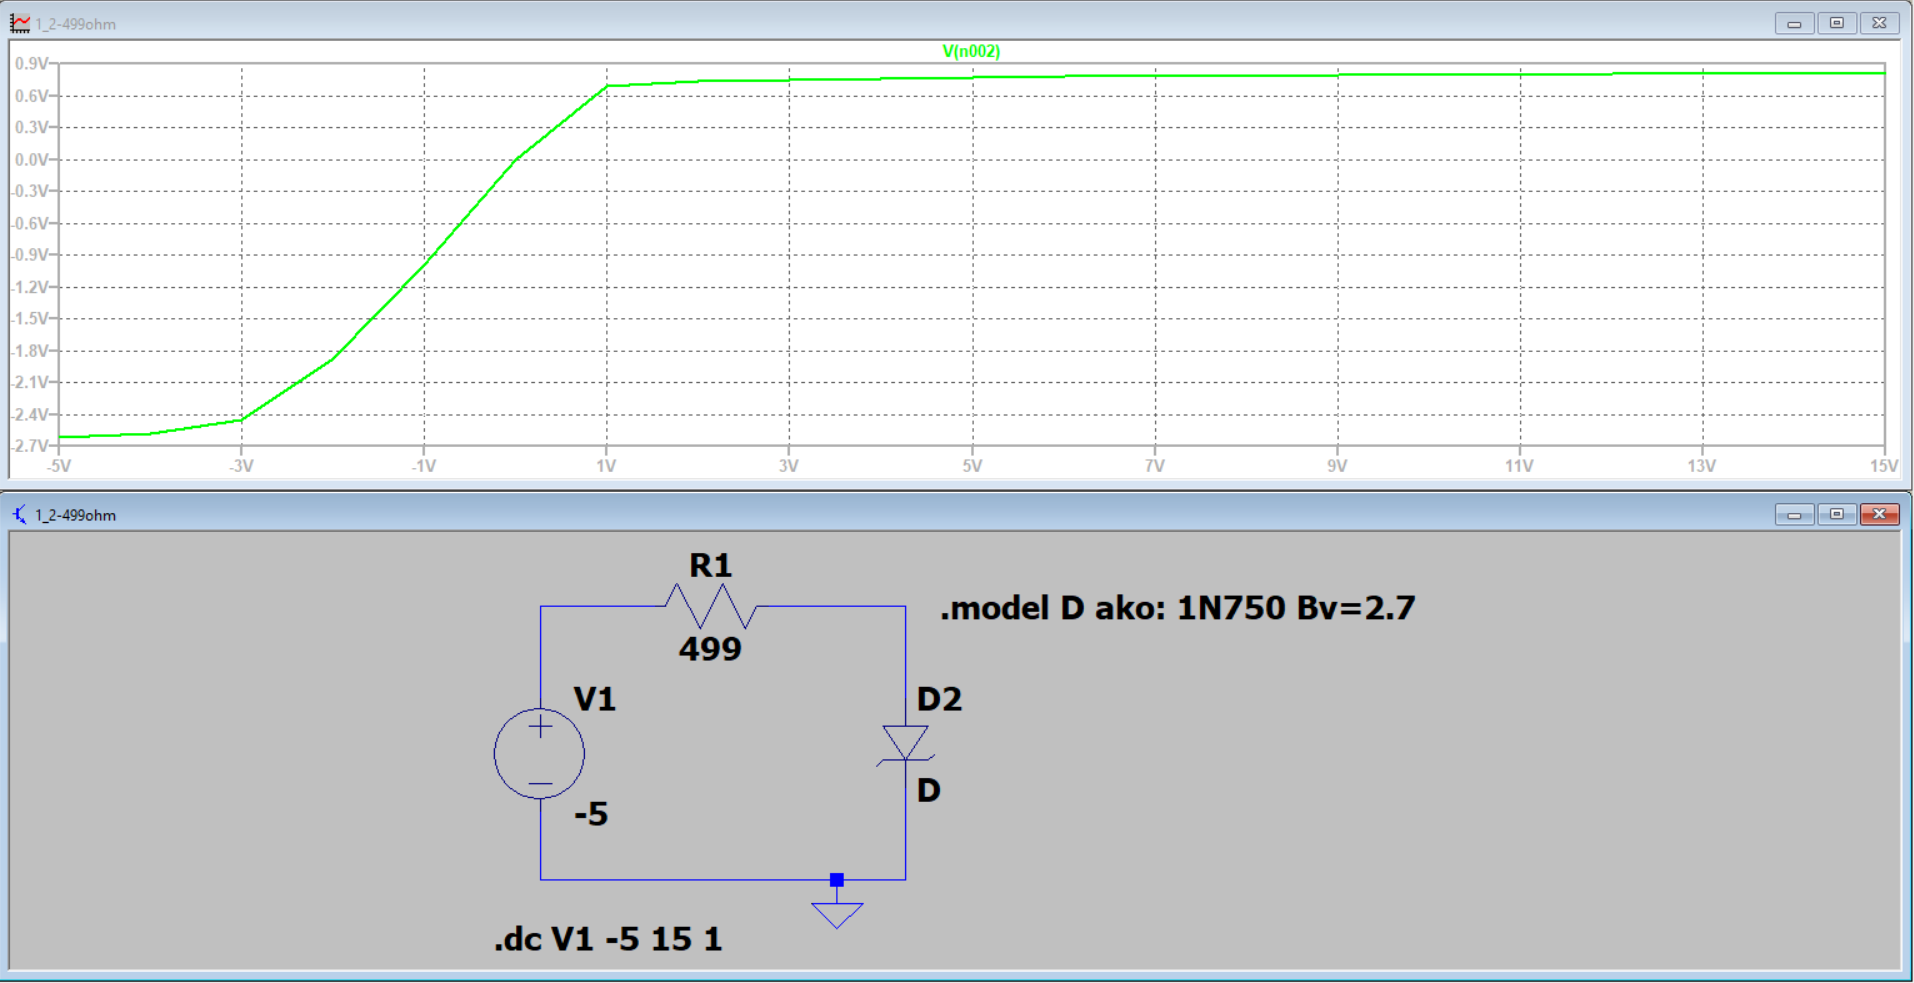
\includegraphics[width=9cm]{Screenshot 2024-07-15 063312}}
		\subfloat[\centering LTSpice + Rudimentary Schematic Series RD ($10k\Omega$) Circuit]{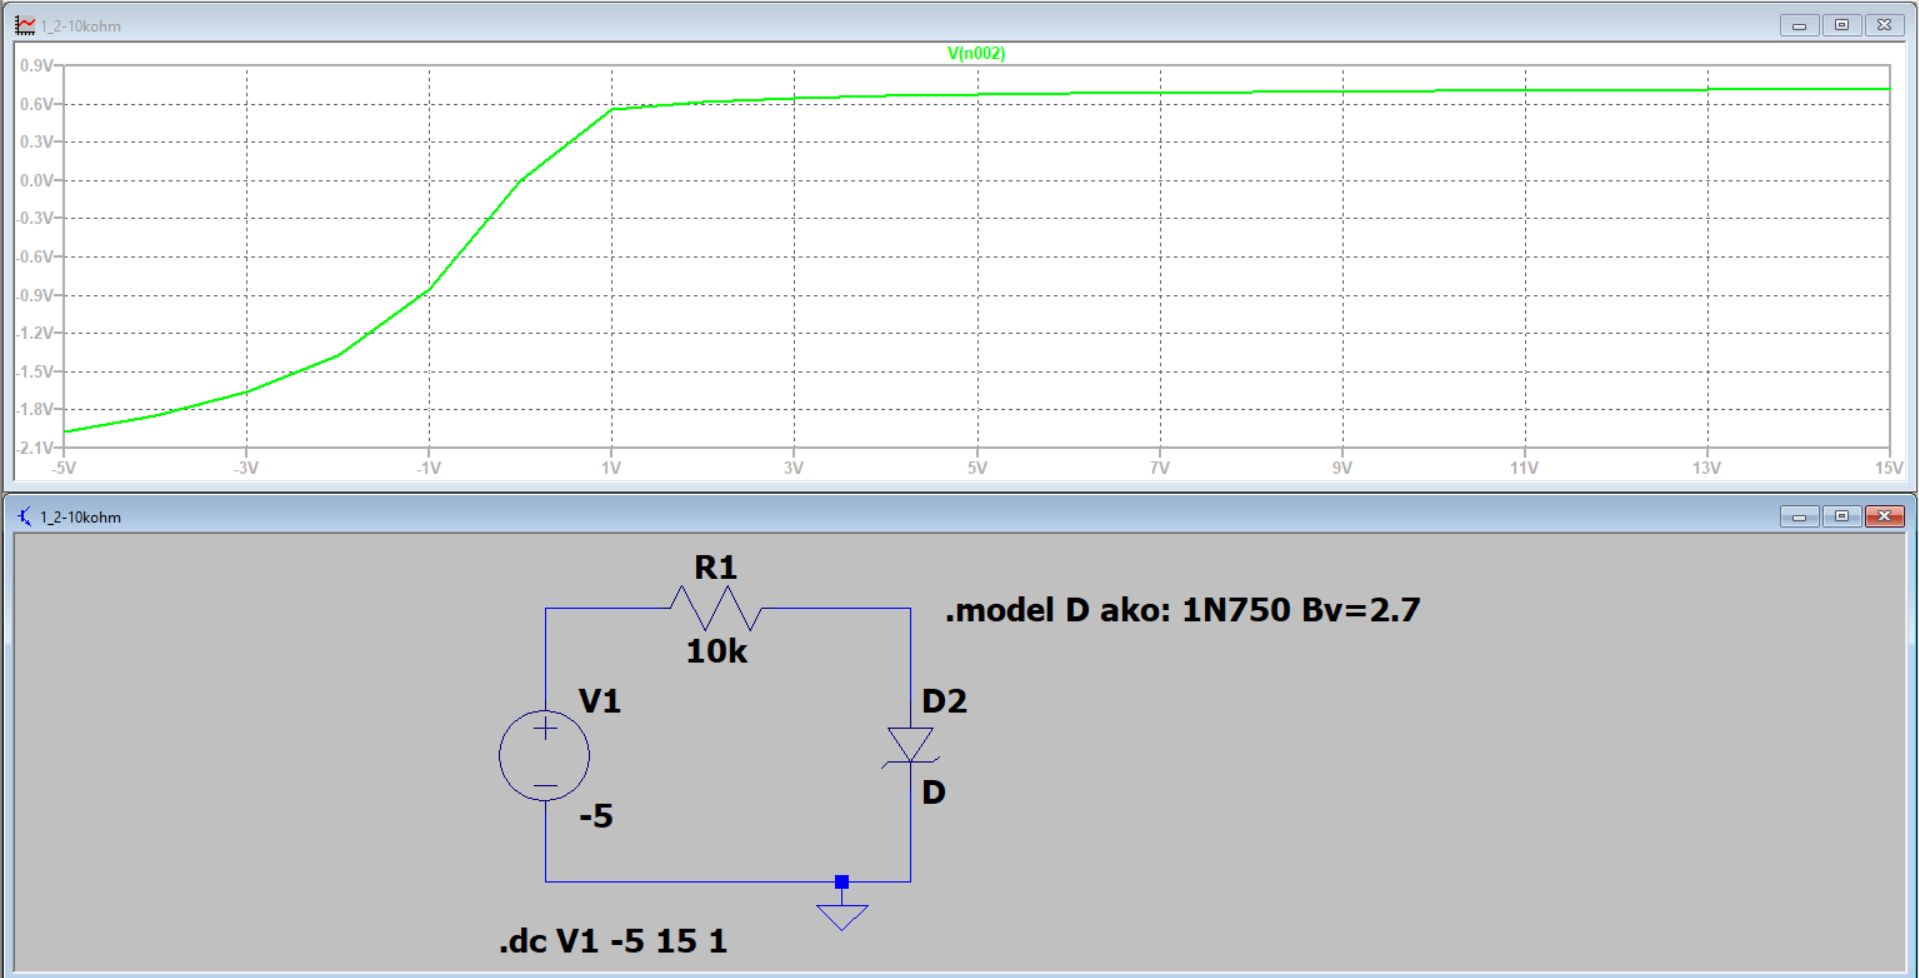
\includegraphics[width=9cm]{Screenshot 2024-07-15 062954}}
	\end{figure}
	\begin{figure}[hp!]
		\ContinuedFloat
		\centering
		\subfloat[\centering Series RD Circuit $499\Omega$]{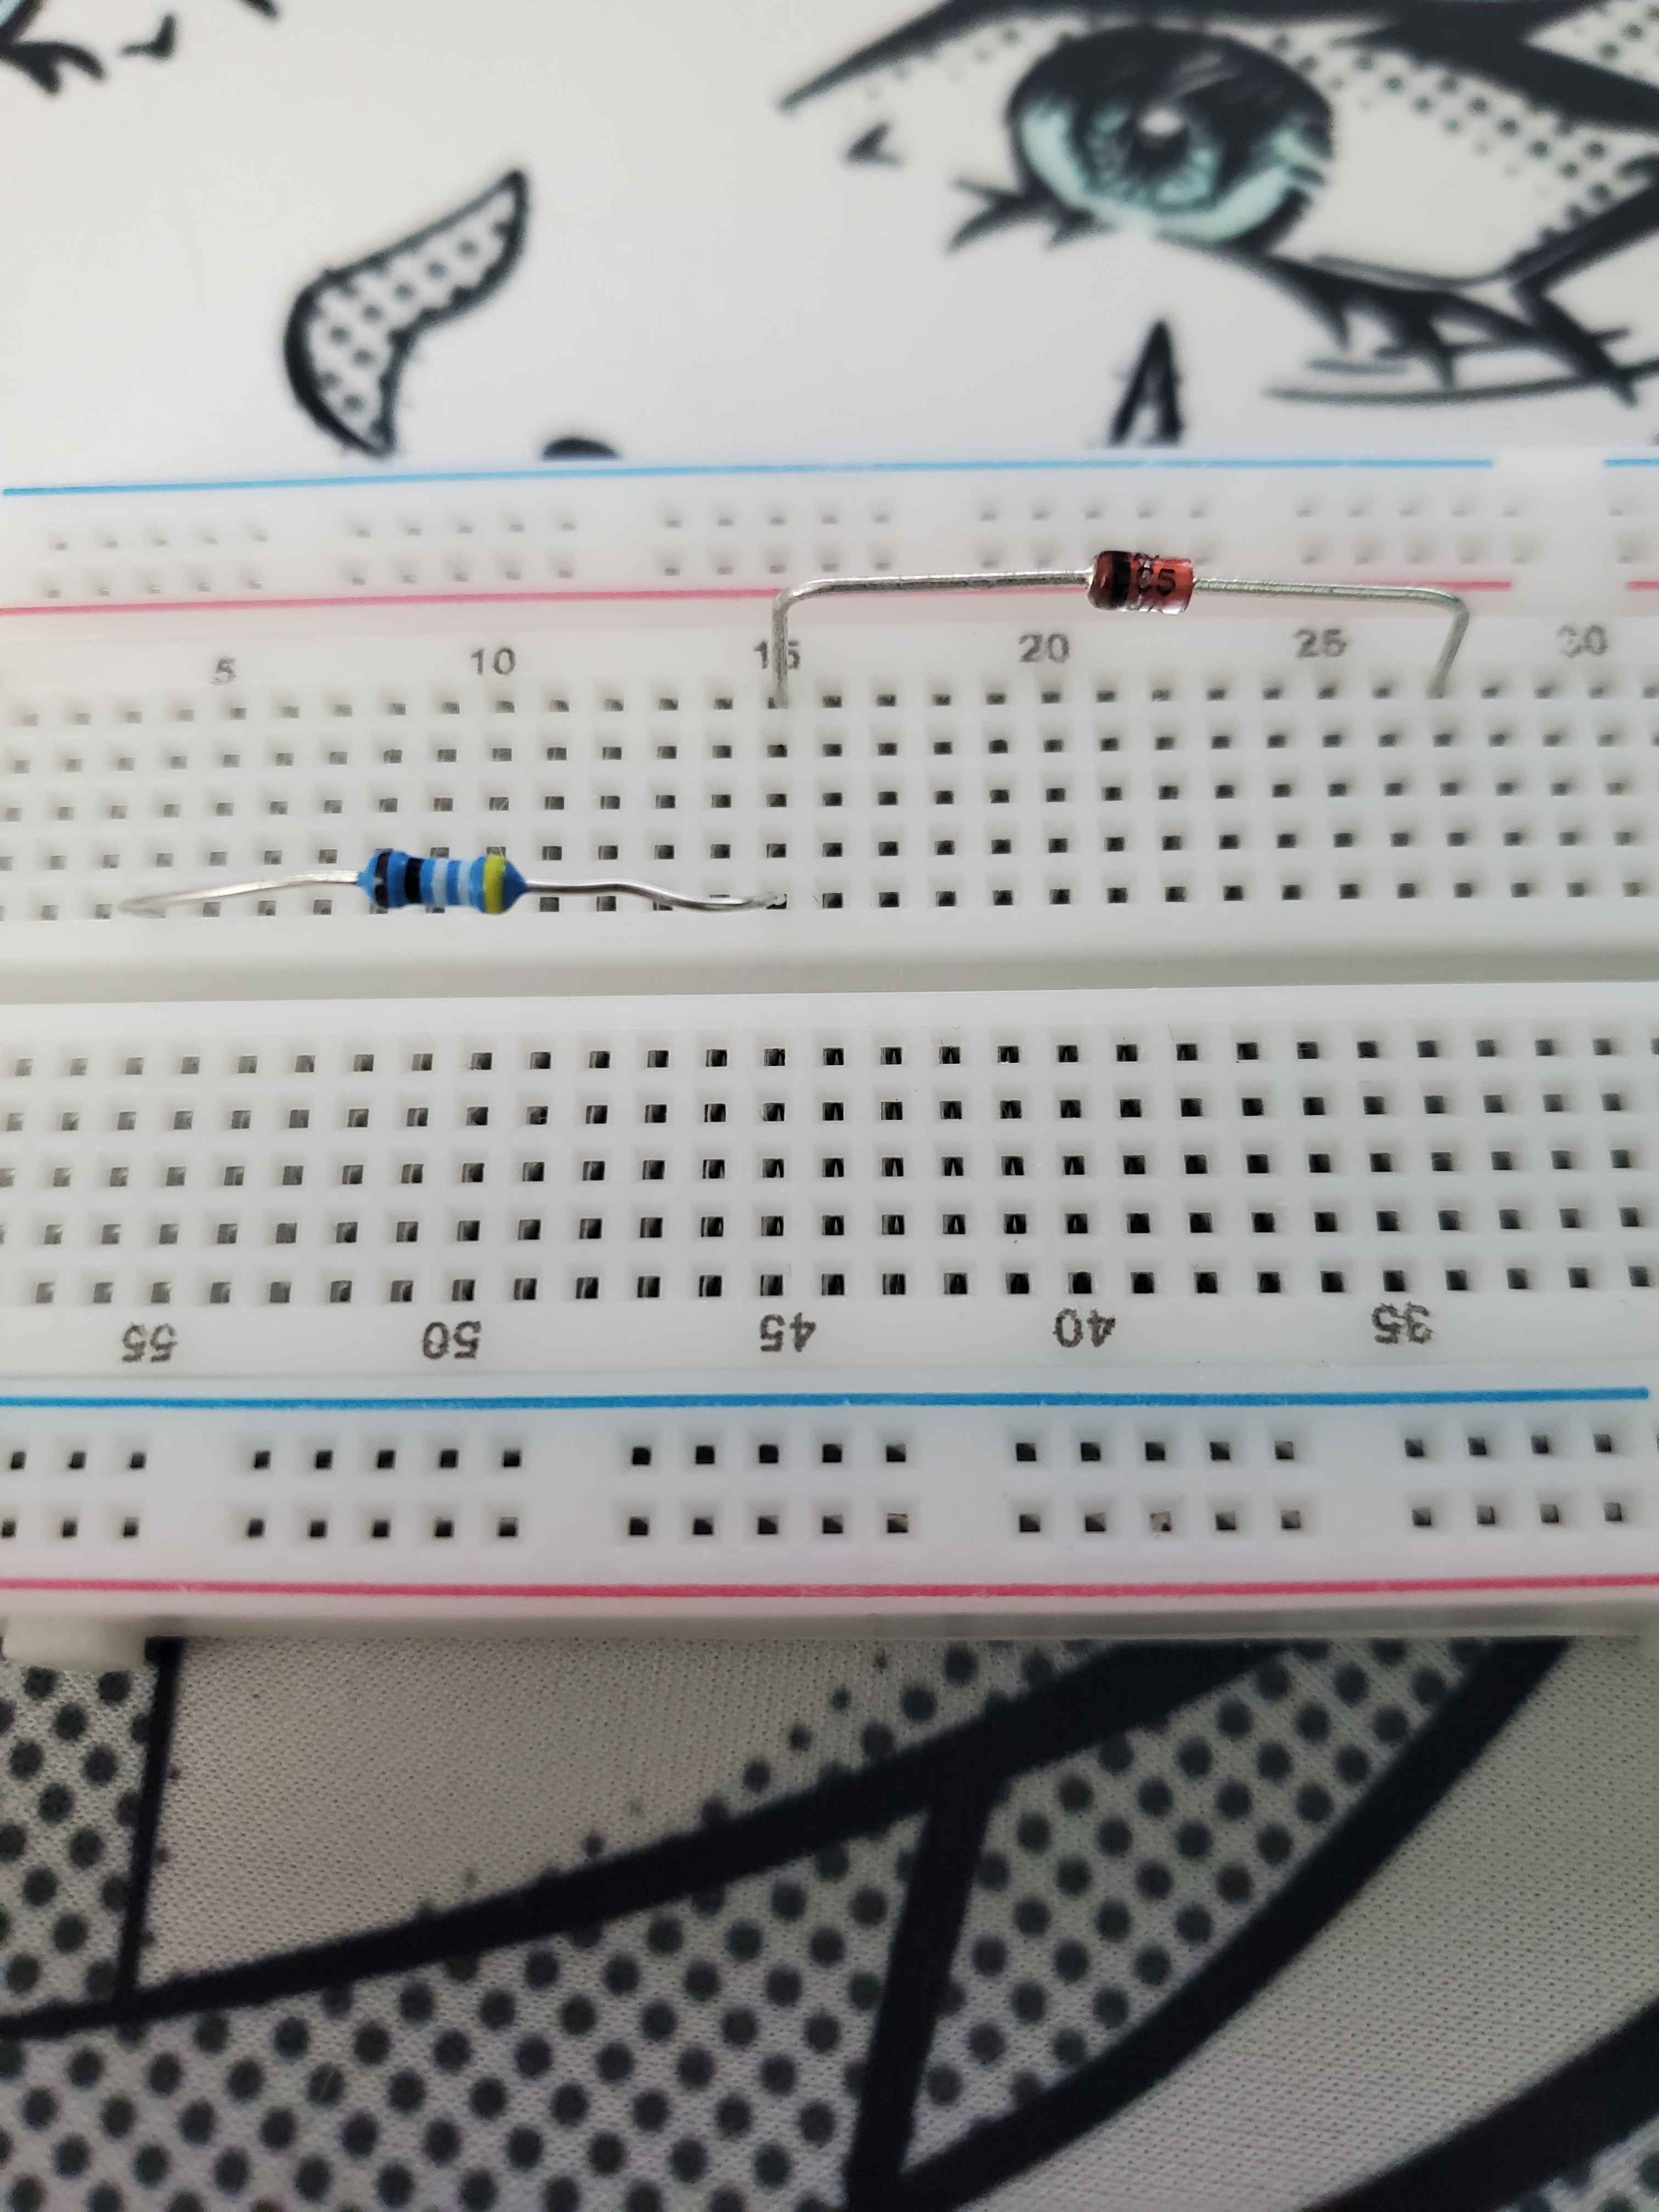
\includegraphics[width=9cm]{20240714_094624}}\hfil
		\subfloat[\centering Series RD Circuit $10k\Omega$]{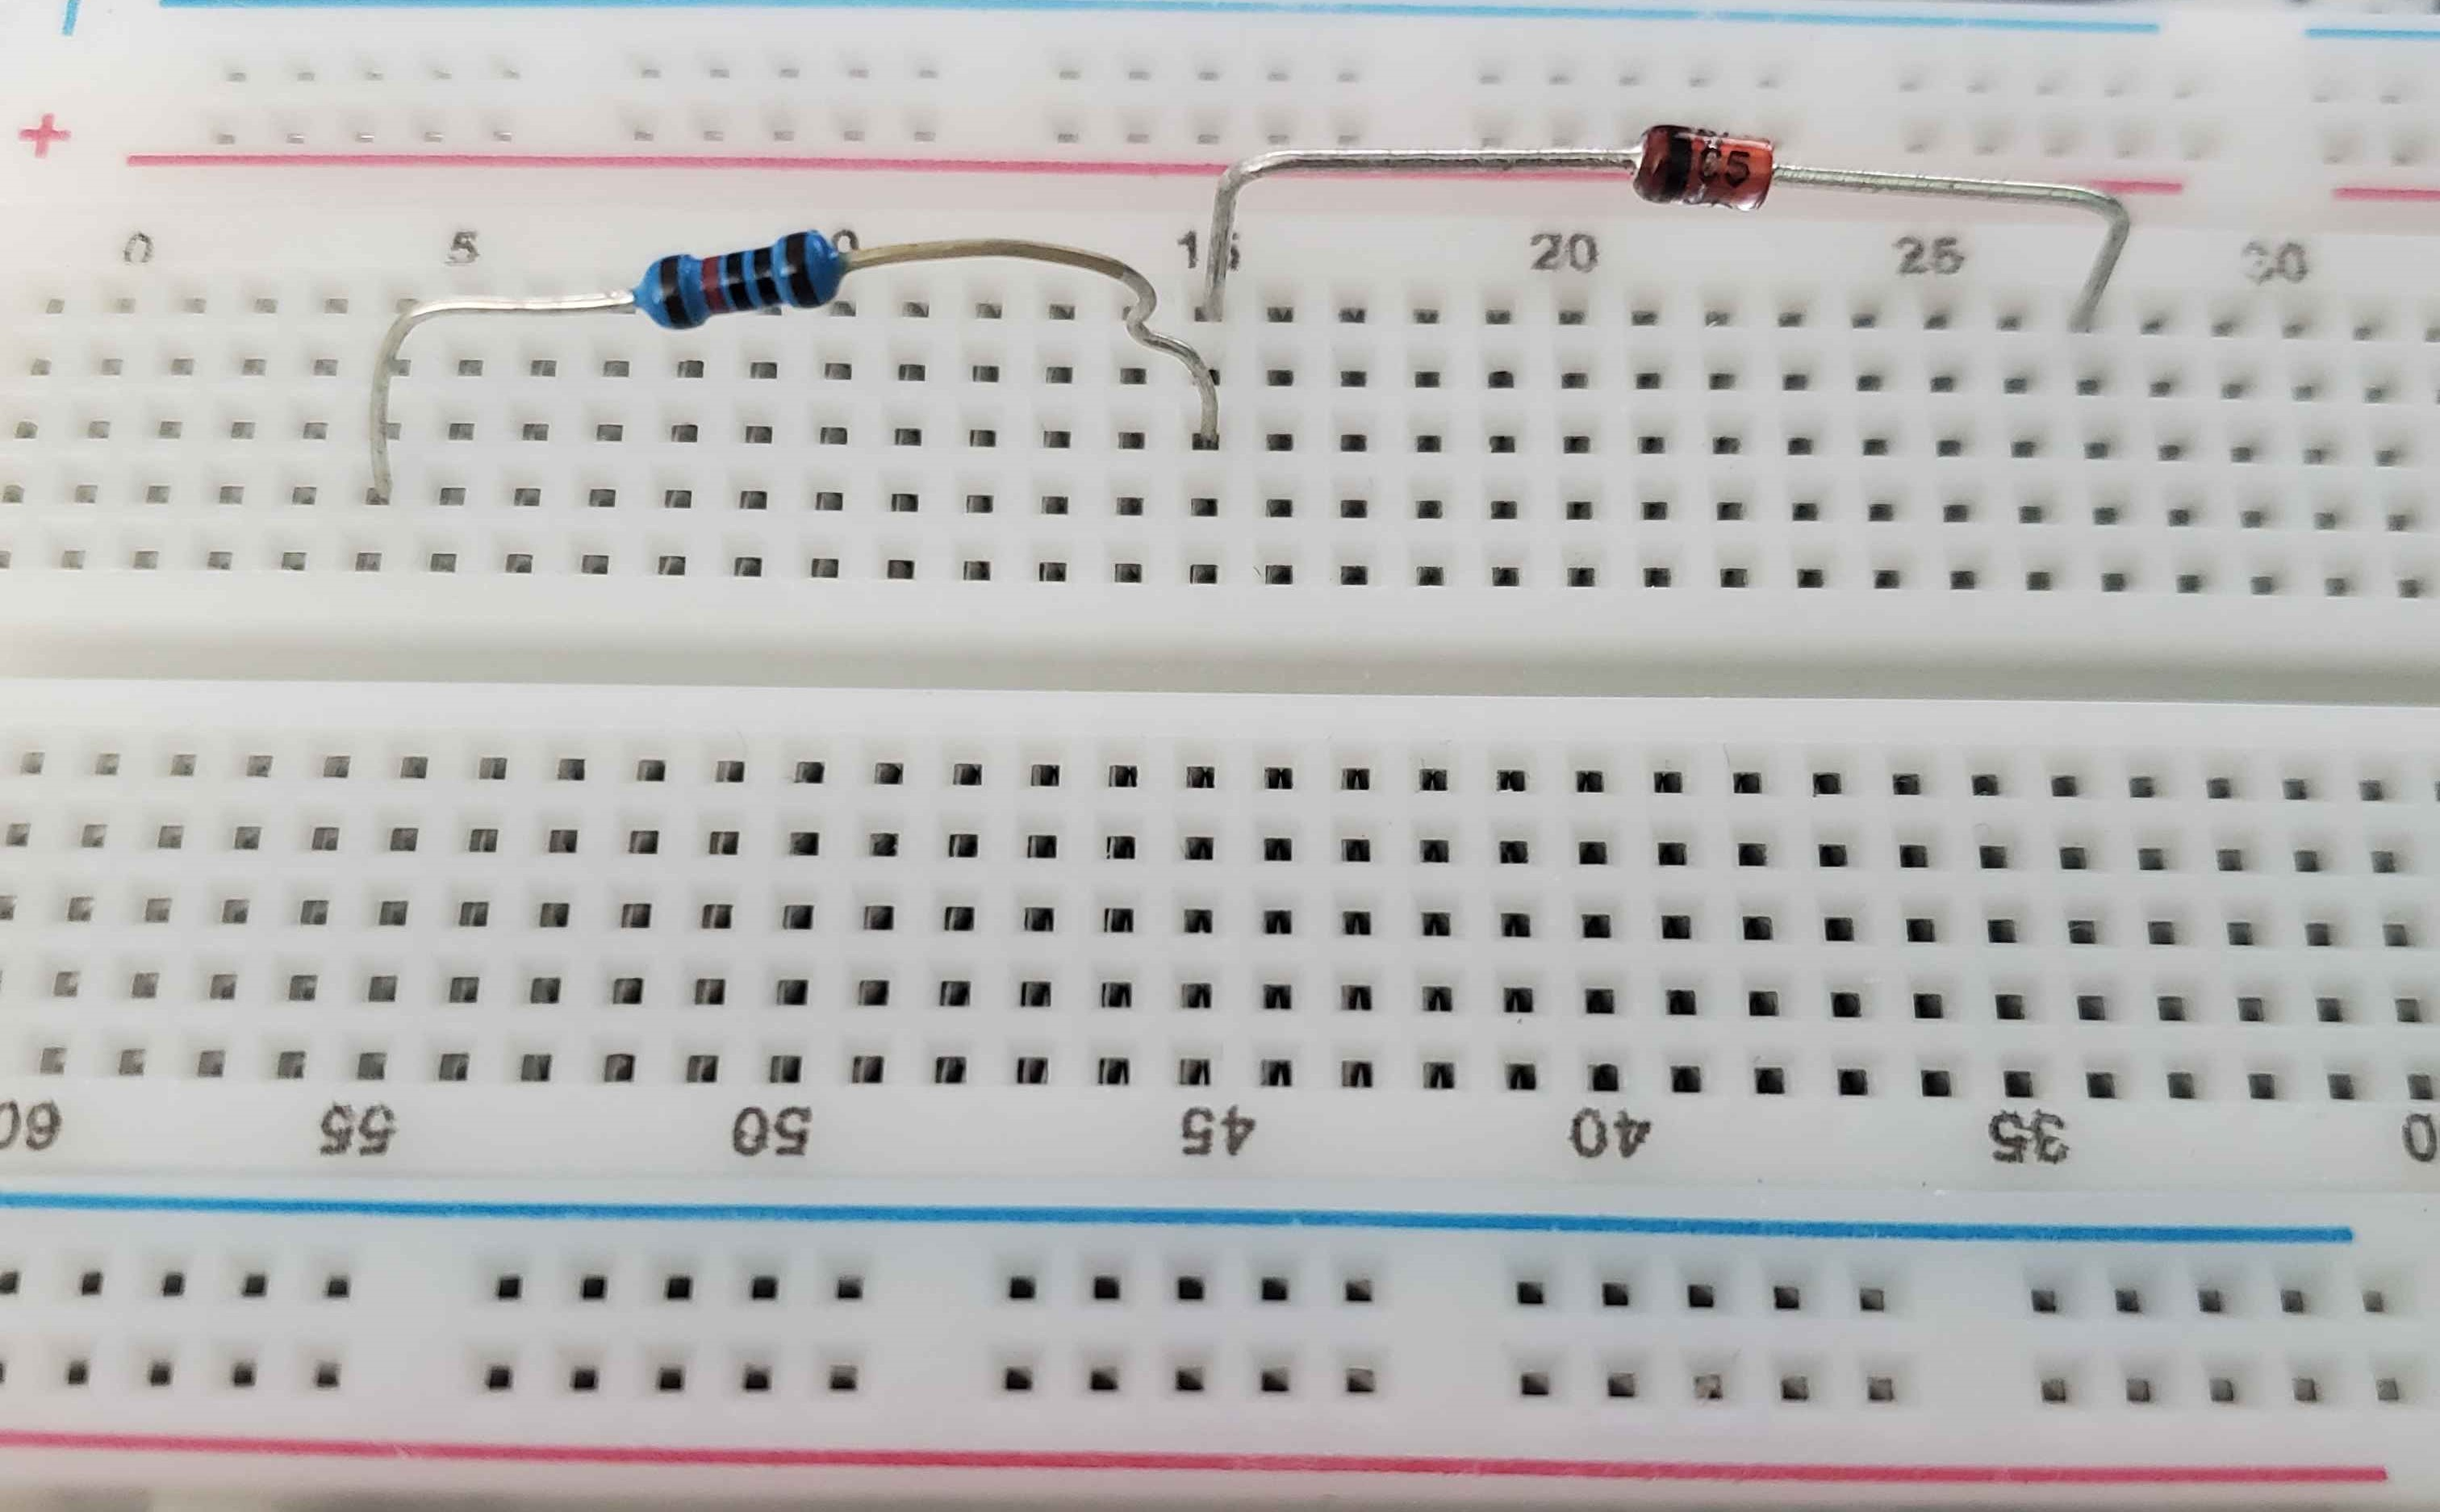
\includegraphics[width=9cm]{20240714_094351}}
	\end{figure}
	\newpage
	\nsection{Descriptions of Measurements \& Calculations}
	Given the default theoretical calculation for a Diode in forward-bias: $I_D=I_S(e^{\frac{V_D}{V_T}}-1)$; the dataset is similar in-nature - not exact because the characteristics of this diode differs - from section 1.1 of the lab.\\
	The characteristic of a \textit{Zener} Diode is its relationship to $-V_D$, as $I_D$ enters \textbf{Reverse-Breakdown} @ $-V_{Z0}$; the point of breakdown.
	\begin{figure}[hp!] %140, 
		\centering
		\caption{$RD_Z$ Circuit}
		\subfloat[RD Circuit Measurement]{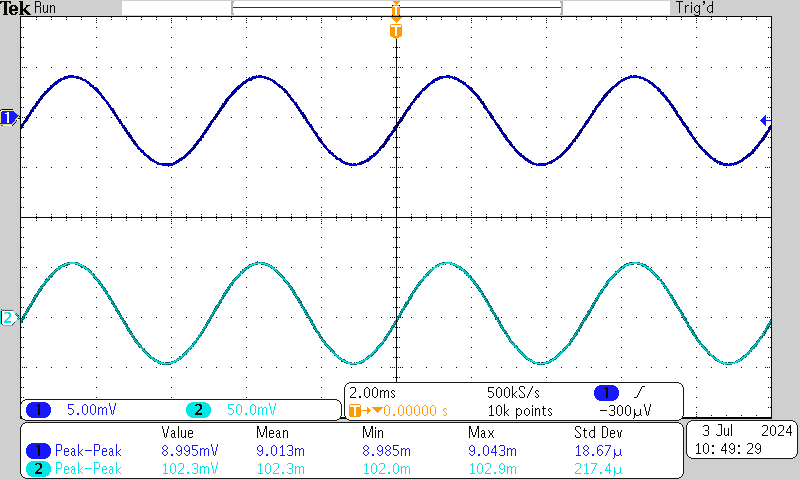
\includegraphics[width=9cm]{tek0000}}
		\subfloat[Sample Measurement ]{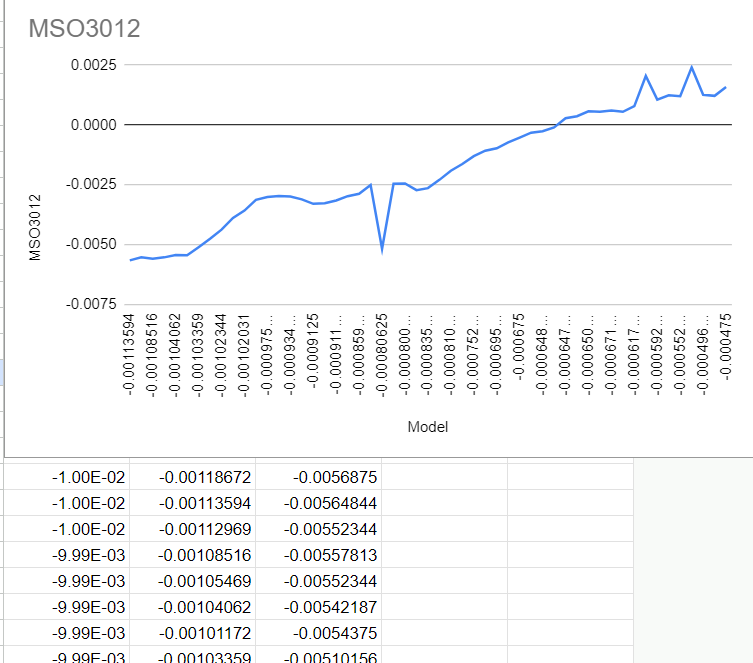
\includegraphics[width=9cm]{Screenshot 2024-07-15 203328}}
	\end{figure}
	\nsection{Summary \& Conclusions}
	Revealed in Figure RD-Circuit 1A \& 1B, the generated oscilloscope readings of the two periodic function match the characteristics of the transfer function found in 1b ($RD_Z$ Circuit). So the measurements do infact closely align.
	\nsubsection{Discussion}
	\begin{itemize}
		\item \textbf{i. Describe how you measured $I_D$ and $V_D$?}
		\subitem At the node where R; ($R>100\Omega$) and the Zener Diode; ($D_Z$) meet, we denote this junction as $V_{out}$. We attach our Multimetre's positive lead (Red) to $V_{out}$, and attached our ground lead to the opposing node of the Zener Diode; ($D_Z$) - which should be grounded.
		\item \textbf{ii. In this experiment how would you determine the value of $I_{D,max}$}
		\subitem \emph{Forward-Bias:} $I_D=I_S(e^{\frac{V_D}{V_T}}-1)$; reference Figure 1b.
		\subitem \emph{Reverse-Breakdown:} The functioning range when $V_D < V_{D_{BR}}$; the output voltage of a reverse-breakdown Zener diode is $V_o=V_i-R_i*_i$ (the subscript of i meaning input of the function generator.)
		\item \textbf{iii. In the circuit, what limits $I_D$?}
		\subitem \emph{Forward-Bias:} The characteristics of the I-V curve of a diode has current $I_D$ exponentially rise towards a cut-off at the threshold, towards the C.V.D @ $V_D$.
		\subitem \emph{Reverse-Breakdown:} Similarly to how the Forward-Bias meets an exponential curve towards its threshold; $V_D$, the Reverse-Breakdown meets and meets a sharp declination of $V_o$ towards $-V_{D_{BR}}$.
		\item \textbf{iv. Explain why $V_D$ does not change much while $I_D$ can change a lot.}
		\subitem Given the equation of a Diode's characteristics of $I_D=I_S(e^{\frac{V_D}{V_T}}-1)$. Putting the equation in reference to $I_D$ is an exponential function, while $V_D$ is a logarithmic function with a very slow rise time. This goes for both Forward-Bias and Reverse-Breakdown, only the output voltage nature changes.
	\end{itemize}
	\newpage
	\newpage
	\nsection{Bibliography}
	\textbf{Cited:}\\
	\begin{itemize}
		\item Lab 1 Manual
		\item Sedra, Adel, and Kenneth Smith. Microelectronic Circuits. S.L., Oxford Univ Press Us, 2019.
		\item “How Do You Calculate, a Silicon Junction Diode with N = 1 Has v = 0.7 v al I = 1 MA. What Is the Voltage Drop at I=0.1 MA and I=10 MA.?” Quora, 2024, appliedmathematics.quora.com/How-to-calculate-A-silicon-junction-diode-with-n-1-has-v-0-7-V-al-I-1-mA-What-is-the-voltage-drop-at-I-0-1-mA-an?top\_ans=223007030. Accessed 15 July 2024.
	\end{itemize}
	\begin{figure}[!h]
		\subfloat[Look at her, she's perfect.]{
\includegraphics[width=\linewidth]{GodILoveFurina}}
	\end{figure}
\end{document}